\begin{longtable} { | c | p{12cm} | c | } 
\hline
	ID 	&	Issues	&		 Es. hours \\\hline
	34 	&	Choices in Sequences		&	16 hours \\\hline
\caption{Issue ID 34}
\label{tab:spr2_nested}
\end{longtable}

The more independent users can easily handle sequences covering a larger timespan. These sort of sequences require a possibility to create nested sequences (e.g. a morning schema could entail smaller sequences such as eat breakfast, or take a shower). Furthermore it is sometimes when the autistics at institutions have a period of free time and they are presented with a choice (e.g. playing with cars or drawing).
This has been solved by allowing the guardian to add already created sequences, as well as choices, instead of only being able to add pictograms. If a sequence is chosen, the user is redirected to a new MainActivity (without all of the buttons), and you can choose from existing sequences. Once a sequence is chosen, it is a nested sequence, i.e. a sequence within another sequence. 

If the user chose to add a choice instead of a sequence or pictogram, he will be presented with another dialogbox. This dialogbox contained a SequenceViewGroup similar to the one in SequenceActivity, where the user is able to add pictograms to the choice. Once the choice is created, the children viewing the finished sequence should be able to make a choice between the added pictograms.

As of the end of sprint 2 the database does not support full sequences which means the full functionality will not be added until sprint 3. This means the issue regarding nested sequences can not be closed completely yet.

\begin{figure} [h!]
\centering
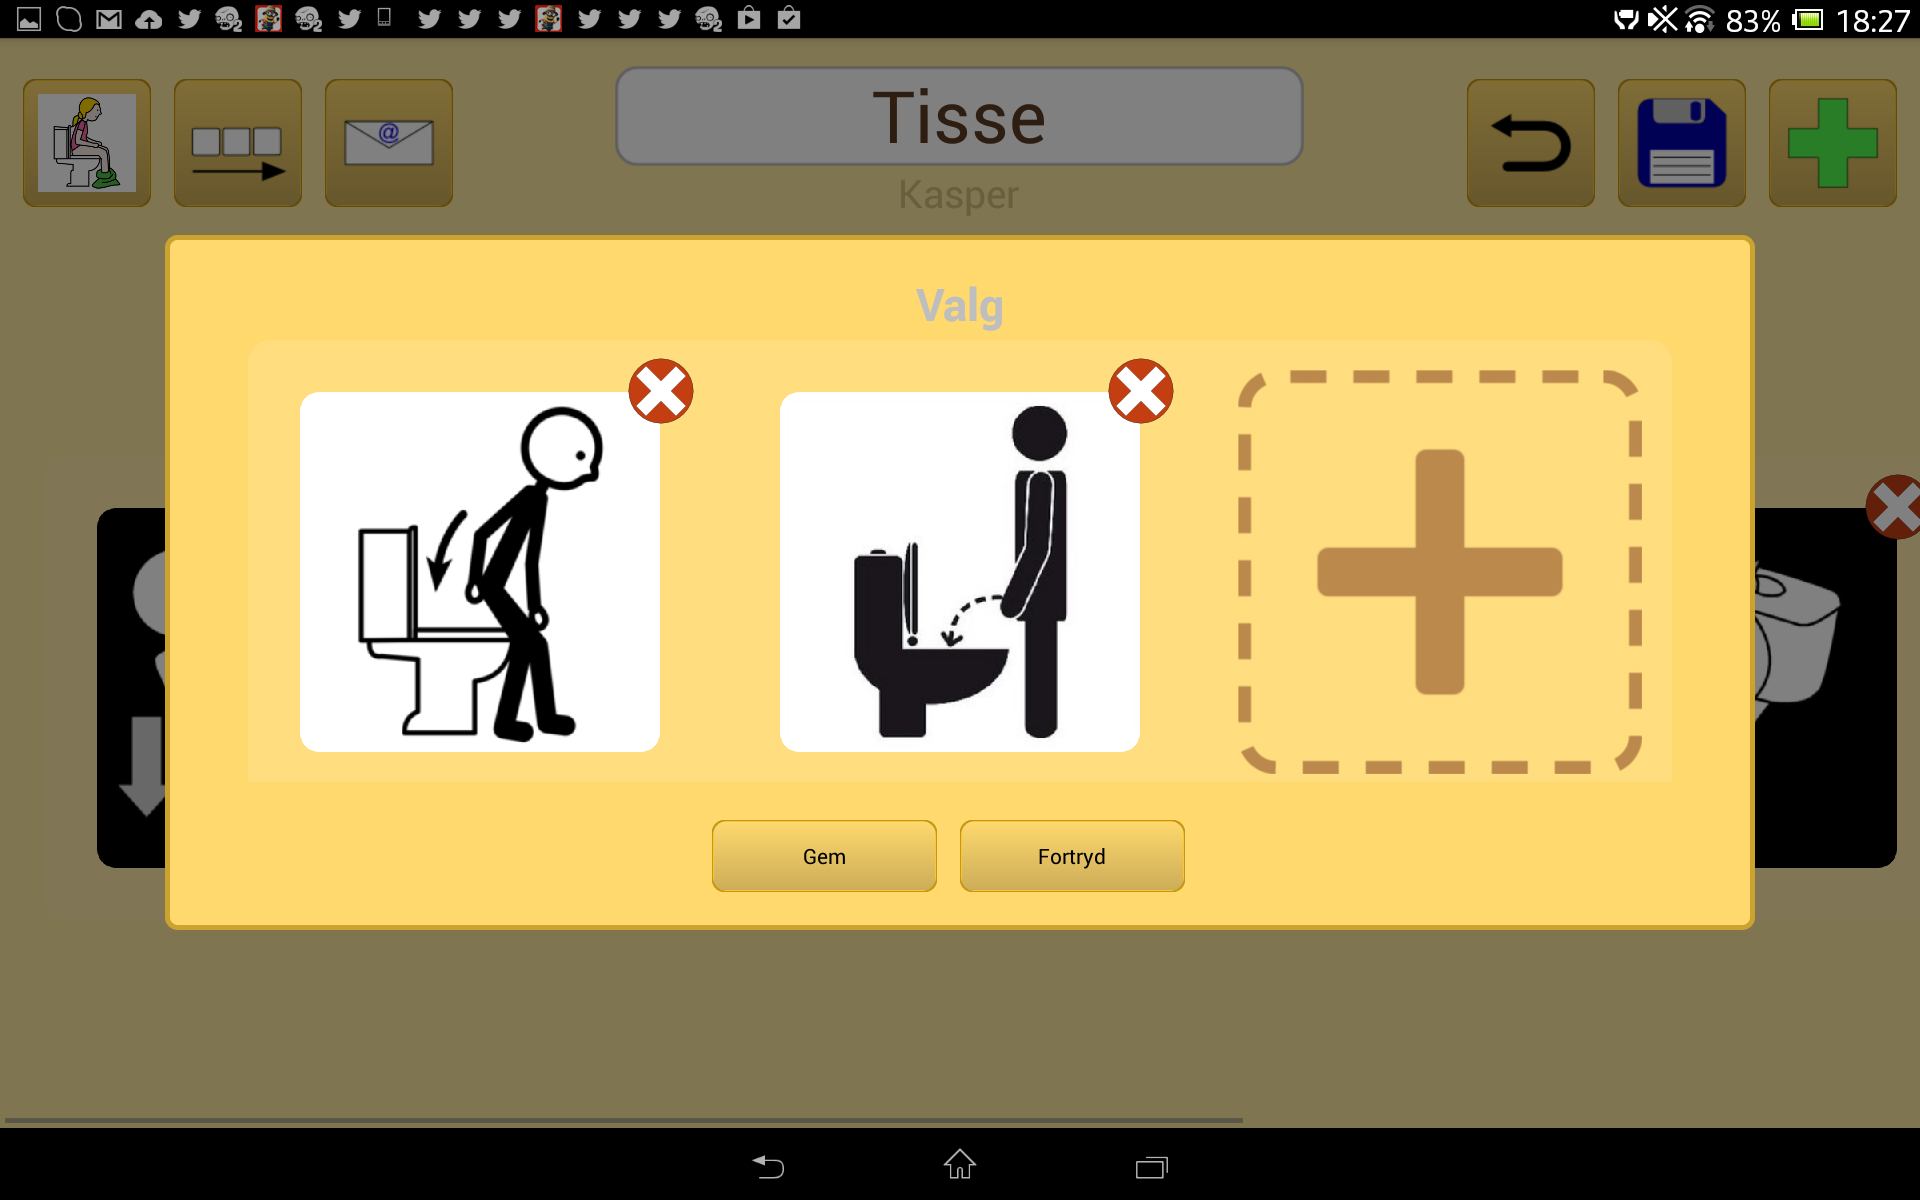
\includegraphics[width=0.95\textwidth]{Pics/Sprint2/choices/choiceDialog.png}
\caption{This is an example of how creating a choice within a sequence}
\label{fig:choiceDialog}
\end{figure}




